% Options for packages loaded elsewhere
\PassOptionsToPackage{unicode}{hyperref}
\PassOptionsToPackage{hyphens}{url}
\PassOptionsToPackage{dvipsnames,svgnames*,x11names*}{xcolor}
%
\documentclass[
]{article}
\usepackage{lmodern}
\usepackage{amssymb,amsmath}
\usepackage{ifxetex,ifluatex}
\ifnum 0\ifxetex 1\fi\ifluatex 1\fi=0 % if pdftex
  \usepackage[T1]{fontenc}
  \usepackage[utf8]{inputenc}
  \usepackage{textcomp} % provide euro and other symbols
\else % if luatex or xetex
  \usepackage{unicode-math}
  \defaultfontfeatures{Scale=MatchLowercase}
  \defaultfontfeatures[\rmfamily]{Ligatures=TeX,Scale=1}
\fi
% Use upquote if available, for straight quotes in verbatim environments
\IfFileExists{upquote.sty}{\usepackage{upquote}}{}
\IfFileExists{microtype.sty}{% use microtype if available
  \usepackage[]{microtype}
  \UseMicrotypeSet[protrusion]{basicmath} % disable protrusion for tt fonts
}{}
\makeatletter
\@ifundefined{KOMAClassName}{% if non-KOMA class
  \IfFileExists{parskip.sty}{%
    \usepackage{parskip}
  }{% else
    \setlength{\parindent}{0pt}
    \setlength{\parskip}{6pt plus 2pt minus 1pt}}
}{% if KOMA class
  \KOMAoptions{parskip=half}}
\makeatother
\usepackage{xcolor}
\IfFileExists{xurl.sty}{\usepackage{xurl}}{} % add URL line breaks if available
\IfFileExists{bookmark.sty}{\usepackage{bookmark}}{\usepackage{hyperref}}
\hypersetup{
  pdftitle={Multi Stage Design Survey},
  pdfauthor={Vasquez Arriaga Jorge},
  colorlinks=true,
  linkcolor=Maroon,
  filecolor=Maroon,
  citecolor=Blue,
  urlcolor=blue,
  pdfcreator={LaTeX via pandoc}}
\urlstyle{same} % disable monospaced font for URLs
\usepackage[margin=1in]{geometry}
\usepackage{color}
\usepackage{fancyvrb}
\newcommand{\VerbBar}{|}
\newcommand{\VERB}{\Verb[commandchars=\\\{\}]}
\DefineVerbatimEnvironment{Highlighting}{Verbatim}{commandchars=\\\{\}}
% Add ',fontsize=\small' for more characters per line
\usepackage{framed}
\definecolor{shadecolor}{RGB}{248,248,248}
\newenvironment{Shaded}{\begin{snugshade}}{\end{snugshade}}
\newcommand{\AlertTok}[1]{\textcolor[rgb]{0.94,0.16,0.16}{#1}}
\newcommand{\AnnotationTok}[1]{\textcolor[rgb]{0.56,0.35,0.01}{\textbf{\textit{#1}}}}
\newcommand{\AttributeTok}[1]{\textcolor[rgb]{0.77,0.63,0.00}{#1}}
\newcommand{\BaseNTok}[1]{\textcolor[rgb]{0.00,0.00,0.81}{#1}}
\newcommand{\BuiltInTok}[1]{#1}
\newcommand{\CharTok}[1]{\textcolor[rgb]{0.31,0.60,0.02}{#1}}
\newcommand{\CommentTok}[1]{\textcolor[rgb]{0.56,0.35,0.01}{\textit{#1}}}
\newcommand{\CommentVarTok}[1]{\textcolor[rgb]{0.56,0.35,0.01}{\textbf{\textit{#1}}}}
\newcommand{\ConstantTok}[1]{\textcolor[rgb]{0.00,0.00,0.00}{#1}}
\newcommand{\ControlFlowTok}[1]{\textcolor[rgb]{0.13,0.29,0.53}{\textbf{#1}}}
\newcommand{\DataTypeTok}[1]{\textcolor[rgb]{0.13,0.29,0.53}{#1}}
\newcommand{\DecValTok}[1]{\textcolor[rgb]{0.00,0.00,0.81}{#1}}
\newcommand{\DocumentationTok}[1]{\textcolor[rgb]{0.56,0.35,0.01}{\textbf{\textit{#1}}}}
\newcommand{\ErrorTok}[1]{\textcolor[rgb]{0.64,0.00,0.00}{\textbf{#1}}}
\newcommand{\ExtensionTok}[1]{#1}
\newcommand{\FloatTok}[1]{\textcolor[rgb]{0.00,0.00,0.81}{#1}}
\newcommand{\FunctionTok}[1]{\textcolor[rgb]{0.00,0.00,0.00}{#1}}
\newcommand{\ImportTok}[1]{#1}
\newcommand{\InformationTok}[1]{\textcolor[rgb]{0.56,0.35,0.01}{\textbf{\textit{#1}}}}
\newcommand{\KeywordTok}[1]{\textcolor[rgb]{0.13,0.29,0.53}{\textbf{#1}}}
\newcommand{\NormalTok}[1]{#1}
\newcommand{\OperatorTok}[1]{\textcolor[rgb]{0.81,0.36,0.00}{\textbf{#1}}}
\newcommand{\OtherTok}[1]{\textcolor[rgb]{0.56,0.35,0.01}{#1}}
\newcommand{\PreprocessorTok}[1]{\textcolor[rgb]{0.56,0.35,0.01}{\textit{#1}}}
\newcommand{\RegionMarkerTok}[1]{#1}
\newcommand{\SpecialCharTok}[1]{\textcolor[rgb]{0.00,0.00,0.00}{#1}}
\newcommand{\SpecialStringTok}[1]{\textcolor[rgb]{0.31,0.60,0.02}{#1}}
\newcommand{\StringTok}[1]{\textcolor[rgb]{0.31,0.60,0.02}{#1}}
\newcommand{\VariableTok}[1]{\textcolor[rgb]{0.00,0.00,0.00}{#1}}
\newcommand{\VerbatimStringTok}[1]{\textcolor[rgb]{0.31,0.60,0.02}{#1}}
\newcommand{\WarningTok}[1]{\textcolor[rgb]{0.56,0.35,0.01}{\textbf{\textit{#1}}}}
\usepackage{graphicx,grffile}
\makeatletter
\def\maxwidth{\ifdim\Gin@nat@width>\linewidth\linewidth\else\Gin@nat@width\fi}
\def\maxheight{\ifdim\Gin@nat@height>\textheight\textheight\else\Gin@nat@height\fi}
\makeatother
% Scale images if necessary, so that they will not overflow the page
% margins by default, and it is still possible to overwrite the defaults
% using explicit options in \includegraphics[width, height, ...]{}
\setkeys{Gin}{width=\maxwidth,height=\maxheight,keepaspectratio}
% Set default figure placement to htbp
\makeatletter
\def\fps@figure{htbp}
\makeatother
\setlength{\emergencystretch}{3em} % prevent overfull lines
\providecommand{\tightlist}{%
  \setlength{\itemsep}{0pt}\setlength{\parskip}{0pt}}
\setcounter{secnumdepth}{-\maxdimen} % remove section numbering
\usepackage[spanish]{babel}
\usepackage[utf8]{inputenc}
\decimalpoint
\usepackage{booktabs}
\usepackage{longtable}
\usepackage{array}
\usepackage{multirow}
\usepackage{wrapfig}
\usepackage{float}
\usepackage{colortbl}
\usepackage{pdflscape}
\usepackage{tabu}
\usepackage{threeparttable}
\usepackage{threeparttablex}
\usepackage[normalem]{ulem}
\usepackage{makecell}
\usepackage{xcolor}
\usepackage{fancyhdr}
\usepackage{lastpage}

\title{Estimación básica de una encuesta con diseño multi-etápico}
\author{Vasquez Arriaga Jorge}
\date{}

\begin{document}
%\maketitle
\thispagestyle{plain}
\hrule
\begin{center}
	\vspace{0.2cm}
	\huge{Encuesta con diseño
		multietápico}\\
	
	\large{Muestreo}
\end{center}

\vspace{0.1cm}

\begin{table}[h]
	\centering
	\begin{tabular}{ll}
		Vasquez Arriaga Jorge 
	\end{tabular}
\end{table}

\hrule

\vspace{5mm}

\setlength{\parindent}{0cm}


\hypertarget{estimaciuxf3n-buxe1sica-de-una-encuesta-con-diseuxf1o-multietuxe1pico}{%
\subsection{1 Estimación básica de una encuesta con diseño
multietápico}\label{estimaciuxf3n-buxe1sica-de-una-encuesta-con-diseuxf1o-multietuxe1pico}}

Considerando la Encuesta Nacional de Vivienda (ENVI) 2020

\url{https://www.inegi.org.mx/programas/envi/2020/}

Se quiere generar los resultados básicos
presentados en el tabulado llamado Cuadro 5.1, ver Figura \ref{Envi2020}
(\url{https://www.inegi.org.mx/contenidos/programas/envi/2020/tabulados/envi_2020_tema_05_xlsx.zip})

En éste proyecto se busca:

\begin{enumerate}
\def\labelenumi{\roman{enumi}.}
\tightlist
\item
  Describir brevemente el diseño de muestreo usado en la encuesta.
%\begin{enumerate}
%\def\labelenumi{\roman{enumi}.}
%\tightlist
\item
  Identificar las variables asociadas al diseño de muestreo que están
  presentes en la base de datos a usar (THOGAR en
  \url{https://www.inegi.org.mx/programas/envi/2020/\#Microdatos})
\item
  Identificar la pregunta y variable asociada a la identificación de los
  Hogares con necesidad de rentar, comprar o construir una vivienda
  independiente de la que habitan.
\item
  Estimar el número total de hogares y el porcentaje de hogares que tienen una necesidad de vivienda a nivel nacional y por entidad federativa.
\item
  Calcular intervalos de confianza para los parámetros estimados en el inciso anterior.
%\item
%   Considerar el porcentaje de hogares que tienen una necesidad de vivienda por entidad federativa, realizar un mapa de calor (Geographic Heat Map).
\end{enumerate}

El código del proyecto se encuentra en \href{https://github.com/arriagajorge/multi-stage-desing-survey}{https://github.com/arriagajorge/multi-stage-desing-survey}.

\begin{figure}[H]
\centering
    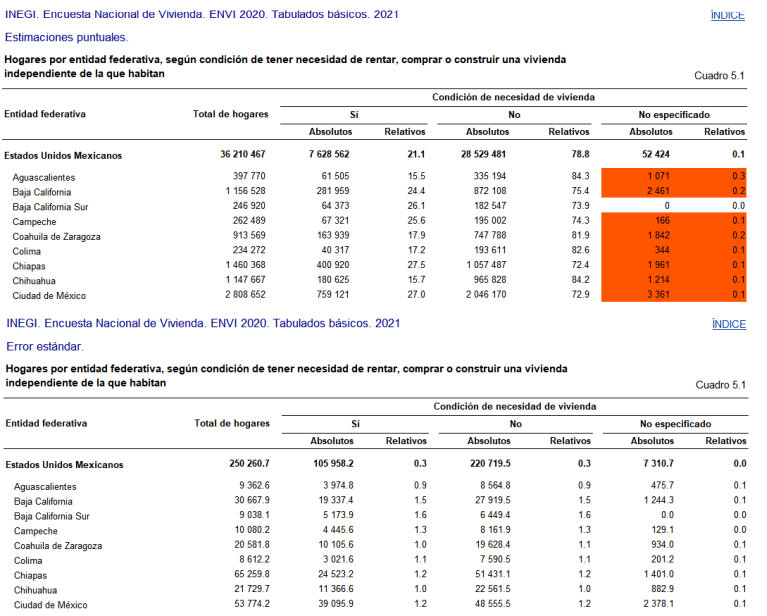
\includegraphics[width=160mm]{images/ENVI2020.png}
    \caption{Parte del cuadro 5.1 de los resultados de la ENVI 2020}
    \label{Envi2020}
\end{figure}

\begin{figure}[H]
\centering
    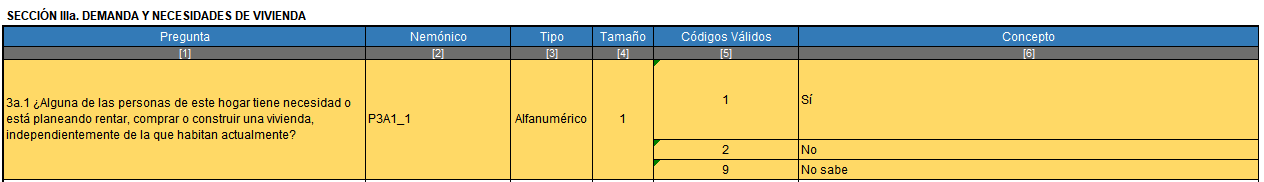
\includegraphics[width=160mm]{images/enc.png}
    \caption{Pregunta de interés, demandas y necesidades de vivienda}
    \label{Pregunta de interés}
\end{figure}

Se usó un diseño probabilístico, cuyo diseño muestral fue bietápico,
donde en la primera etapa se usó un diseño de muestreo estratificado y
en la segunda etapa un diseño de muestreo por conglomerados.

A continuación se muestra el código en \texttt{R}, usado para replicar los resultados.

\begin{Shaded}
\begin{Highlighting}[]
\CommentTok{# leer la base de datos}

\NormalTok{thogar <-}\StringTok{ }\NormalTok{data.table}\OperatorTok{::}\KeywordTok{fread}\NormalTok{(}\StringTok{"THOGAR.csv"}\NormalTok{)}

\CommentTok{# P3A1_1 es la variable a la que nos interesa replicar la estimación}
\CommentTok{# primero observamos que no hay N.A. por lo cual no es necesario hacer correciones}
\NormalTok{thogar2 <-}\StringTok{ }\NormalTok{thogar }\OperatorTok\StringTok{ }\KeywordTok{drop_na}\NormalTok{(P3A1_}\DecValTok{1}\NormalTok{)}
\KeywordTok{length}\NormalTok{(thogar2}\OperatorTok{$}\NormalTok{P3A1_}\DecValTok{1}\NormalTok{) }\OperatorTok{==}\StringTok{ }\KeywordTok{length}\NormalTok{(thogar}\OperatorTok{$}\NormalTok{P3A1_}\DecValTok{1}\NormalTok{)}
\end{Highlighting}
\end{Shaded}

\begin{verbatim}
## [1] TRUE
\end{verbatim}

\begin{Shaded}
\begin{Highlighting}[]
\CommentTok{# un vistazo a las variables que usaremos en el diseño muestral}
\KeywordTok{summary}\NormalTok{(thogar[, }\KeywordTok{c}\NormalTok{(}\StringTok{"UPM_DIS"}\NormalTok{, }\StringTok{"EST_DIS"}\NormalTok{, }\StringTok{"FACTOR"}\NormalTok{)])}
\end{Highlighting}
\end{Shaded}

\begin{verbatim}
##     UPM_DIS            EST_DIS             FACTOR         
##  Min.   :   1.000   Min.   :  1.0000   Min.   :   4.0000  
##  1st Qu.:2254.000   1st Qu.:135.0000   1st Qu.: 254.0000  
##  Median :4291.500   Median :268.0000   Median : 473.0000  
##  Mean   :4306.808   Mean   :267.6786   Mean   : 640.0097  
##  3rd Qu.:6329.000   3rd Qu.:397.0000   3rd Qu.: 788.0000  
##  Max.   :8301.000   Max.   :552.0000   Max.   :8610.0000
\end{verbatim}

\begin{Shaded}
\begin{Highlighting}[]
\CommentTok{# segun la estructura de archivo}
\CommentTok{# el número 1 corresponde a si tienen necesidad}
\NormalTok{a <-}\StringTok{ }\KeywordTok{sum}\NormalTok{(thogar}\OperatorTok{$}\NormalTok{P3A1_}\DecValTok{1} \OperatorTok{==}\StringTok{ }\DecValTok{1}\NormalTok{)}
\CommentTok{# el número 2 a los que no}
\NormalTok{b <-}\StringTok{ }\KeywordTok{sum}\NormalTok{(thogar}\OperatorTok{$}\NormalTok{P3A1_}\DecValTok{1} \OperatorTok{==}\StringTok{ }\DecValTok{2}\NormalTok{)}
\CommentTok{# el número 3 a los que no especificaron}
\NormalTok{c <-}\StringTok{ }\KeywordTok{sum}\NormalTok{(thogar}\OperatorTok{$}\NormalTok{P3A1_}\DecValTok{1} \OperatorTok{==}\StringTok{ }\DecValTok{9}\NormalTok{)}
\CommentTok{# efectivamente estos son los únicos resultados}
\KeywordTok{sum}\NormalTok{(a }\OperatorTok{+}\StringTok{ }\NormalTok{b }\OperatorTok{+}\StringTok{ }\NormalTok{c) }\OperatorTok{==}\StringTok{ }\KeywordTok{length}\NormalTok{(thogar}\OperatorTok{$}\NormalTok{P3A1_}\DecValTok{1}\NormalTok{)}
\end{Highlighting}
\end{Shaded}

\begin{verbatim}
## [1] TRUE
\end{verbatim}

\begin{Shaded}
\begin{Highlighting}[]
\CommentTok{# añadimos estos valores al dataframe}
\CommentTok{# los que tienen necesida}
\NormalTok{thogar}\OperatorTok{$}\NormalTok{si <-}\StringTok{ }\KeywordTok{as.numeric}\NormalTok{(thogar}\OperatorTok{$}\NormalTok{P3A1_}\DecValTok{1} \OperatorTok{==}\StringTok{ }\DecValTok{1}\NormalTok{)}
\CommentTok{# los que no tienen necesidad}
\NormalTok{thogar}\OperatorTok{$}\NormalTok{no <-}\StringTok{ }\KeywordTok{as.numeric}\NormalTok{(thogar}\OperatorTok{$}\NormalTok{P3A1_}\DecValTok{1} \OperatorTok{==}\StringTok{ }\DecValTok{2}\NormalTok{)}
\CommentTok{# los que no especificaran}
\NormalTok{thogar}\OperatorTok{$}\NormalTok{ne <-}\StringTok{ }\KeywordTok{as.numeric}\NormalTok{(thogar}\OperatorTok{$}\NormalTok{P3A1_}\DecValTok{1} \OperatorTok{==}\StringTok{ }\DecValTok{9}\NormalTok{)}
\CommentTok{# ocuparemos un vector de unos para calcular el total}
\NormalTok{thogar}\OperatorTok{$}\NormalTok{total <-}\StringTok{ }\DecValTok{1}

\KeywordTok{library}\NormalTok{(survey)}
\CommentTok{# en muchos casos sólo hay una upm en cada estrato, lo que }
\CommentTok{# dificulta la estimación de la varianza por esto ocupamos esta opción}
\KeywordTok{options}\NormalTok{(}\DataTypeTok{survey.lonely.psu=}\StringTok{"adjust"}\NormalTok{)}
\CommentTok{# usamos nest=TRUE ya que no hay seguridad de que las claves de las UPM son únicas}

\CommentTok{# definimos el diseño}
\NormalTok{dsg.envi <-}\StringTok{ }\KeywordTok{svydesign}\NormalTok{(}\DataTypeTok{id=}\OperatorTok{~}\NormalTok{UPM_DIS, }\DataTypeTok{strat=}\OperatorTok{~}\NormalTok{EST_DIS, }\DataTypeTok{weight =}\OperatorTok{~}\NormalTok{FACTOR,}
                      \DataTypeTok{data =}\NormalTok{ thogar, }\DataTypeTok{nest=}\NormalTok{T)}
\CommentTok{# summary(dsg.envi)}

\CommentTok{# guardamos los resultados}
\CommentTok{# por nivel nacional}
\NormalTok{rel.nac <-}\StringTok{ }\KeywordTok{svymean}\NormalTok{(}\OperatorTok{~}\NormalTok{si }\OperatorTok{+}\StringTok{ }\NormalTok{no }\OperatorTok{+}\StringTok{ }\NormalTok{ne, dsg.envi)}\OperatorTok{*}\DecValTok{100}
\NormalTok{abs.nac <-}\StringTok{ }\KeywordTok{svytotal}\NormalTok{(}\OperatorTok{~}\NormalTok{si }\OperatorTok{+}\StringTok{ }\NormalTok{no }\OperatorTok{+}\StringTok{ }\NormalTok{ne, dsg.envi)}
\NormalTok{total.nac <-}\StringTok{ }\KeywordTok{svytotal}\NormalTok{(}\OperatorTok{~}\NormalTok{total, dsg.envi)}

\CommentTok{# por entidadad }
\NormalTok{rel.ent <-}\StringTok{ }\KeywordTok{svyby}\NormalTok{(}\OperatorTok{~}\NormalTok{si }\OperatorTok{+}\NormalTok{no }\OperatorTok{+}\StringTok{ }\NormalTok{ne,}\OperatorTok{~}\NormalTok{ENT,}\DataTypeTok{design=}\NormalTok{dsg.envi, svymean)}
\NormalTok{abs.ent <-}\StringTok{ }\KeywordTok{svyby}\NormalTok{(}\OperatorTok{~}\NormalTok{si}\OperatorTok{+}\StringTok{ }\NormalTok{no }\OperatorTok{+}\StringTok{ }\NormalTok{ne,}\OperatorTok{~}\NormalTok{ENT,}\DataTypeTok{design=}\NormalTok{dsg.envi, svytotal)}
\NormalTok{total.ent <-}\StringTok{ }\KeywordTok{svyby}\NormalTok{(}\OperatorTok{~}\NormalTok{total, }\OperatorTok{~}\NormalTok{ENT,}\DataTypeTok{design=}\NormalTok{dsg.envi, svytotal)}

\CommentTok{#anexar los nombres de las entidades (para hacer las tablas)}
\NormalTok{entidades=}\KeywordTok{c}\NormalTok{(}\StringTok{"AGU"}\NormalTok{, }\StringTok{"BCN"}\NormalTok{, }\StringTok{"BCS"}\NormalTok{, }\StringTok{"CAM"}\NormalTok{, }\StringTok{"COA"}\NormalTok{, }\StringTok{"COL"}\NormalTok{, }\StringTok{"CHP"}\NormalTok{, }\StringTok{"CHH"}\NormalTok{, }\StringTok{"CMX"}\NormalTok{, }
            \StringTok{"DUR"}\NormalTok{, }\StringTok{"GUA"}\NormalTok{, }\StringTok{"GRO"}\NormalTok{, }\StringTok{"HID"}\NormalTok{, }\StringTok{"JAL"}\NormalTok{, }\StringTok{"MEX"}\NormalTok{, }\StringTok{"MIC"}\NormalTok{, }\StringTok{"MOR"}\NormalTok{, }\StringTok{"NAY"}\NormalTok{, }\StringTok{"NLE"}\NormalTok{,}
            \StringTok{"OAX"}\NormalTok{, }\StringTok{"PUE"}\NormalTok{, }\StringTok{"QUE"}\NormalTok{, }\StringTok{"ROO"}\NormalTok{, }\StringTok{"SLP"}\NormalTok{, }\StringTok{"SIN"}\NormalTok{, }\StringTok{"SON"}\NormalTok{, }\StringTok{"TAB"}\NormalTok{, }\StringTok{"TAM"}\NormalTok{, }\StringTok{"TLA"}\NormalTok{,}
            \StringTok{"VER"}\NormalTok{, }\StringTok{"YUC"}\NormalTok{, }\StringTok{"ZAC"}\NormalTok{)}

\CommentTok{#mostramos los resultados}
\end{Highlighting}
\end{Shaded}

\begin{Shaded}
\begin{Highlighting}[]
\NormalTok{total.nacdf <-}\StringTok{ }\KeywordTok{as.data.frame}\NormalTok{(total.nac)}
\KeywordTok{colnames}\NormalTok{(total.nacdf) <-}\StringTok{ }\KeywordTok{c}\NormalTok{(}\StringTok{"total"}\NormalTok{, }\StringTok{"se"}\NormalTok{)}
\KeywordTok{row.names}\NormalTok{(total.nacdf) <-}\StringTok{ }\KeywordTok{c}\NormalTok{(}\StringTok{"Nivel nacional"}\NormalTok{)}

\NormalTok{total.entdf <-}\StringTok{ }\NormalTok{total.ent[, }\KeywordTok{c}\NormalTok{(}\StringTok{"total"}\NormalTok{, }\StringTok{"se"}\NormalTok{)]}
\KeywordTok{row.names}\NormalTok{(total.entdf) <-}\StringTok{ }\NormalTok{entidades}

\NormalTok{dftotal <-}\StringTok{ }\KeywordTok{union_all}\NormalTok{(total.nacdf, total.entdf)}
\KeywordTok{colnames}\NormalTok{(dftotal) <-}\StringTok{ }\KeywordTok{c}\NormalTok{(}\StringTok{"Total"}\NormalTok{, }\StringTok{"Error estándar"}\NormalTok{)}

\KeywordTok{kbl}\NormalTok{(dftotal, }\DataTypeTok{caption =} \StringTok{"Total de hogares"}\NormalTok{, }\DataTypeTok{booktabs =}\NormalTok{ T) }\OperatorTok\StringTok{ }
\StringTok{  }\KeywordTok{kable_styling}\NormalTok{(}\DataTypeTok{latex_options =} \KeywordTok{c}\NormalTok{(}\StringTok{"striped"}\NormalTok{, }\StringTok{"HOLD_position"}\NormalTok{))}
\end{Highlighting}
\end{Shaded}

\begin{table}[H]

\caption{\label{tab:unnamed-chunk-13}Total de hogares}
\centering
\begin{tabular}[t]{lrr}
\toprule
  & Total & Error estándar\\
\midrule
\cellcolor{gray!6}{Nivel nacional} & \cellcolor{gray!6}{36210467} & \cellcolor{gray!6}{250260.723090}\\
AGU & 397770 & 9362.560429\\
\cellcolor{gray!6}{BCN} & \cellcolor{gray!6}{1156528} & \cellcolor{gray!6}{30667.900587}\\
BCS & 246920 & 9038.064657\\
\cellcolor{gray!6}{CAM} & \cellcolor{gray!6}{262489} & \cellcolor{gray!6}{10080.177465}\\
\addlinespace
COA & 913569 & 20581.753539\\
\cellcolor{gray!6}{COL} & \cellcolor{gray!6}{234272} & \cellcolor{gray!6}{8612.212124}\\
CHP & 1460368 & 65259.754453\\
\cellcolor{gray!6}{CHH} & \cellcolor{gray!6}{1147667} & \cellcolor{gray!6}{21729.674891}\\
CMX & 2808652 & 53774.155230\\
\addlinespace
\cellcolor{gray!6}{DUR} & \cellcolor{gray!6}{507158} & \cellcolor{gray!6}{12451.339215}\\
GUA & 1663749 & 43662.953028\\
\cellcolor{gray!6}{GRO} & \cellcolor{gray!6}{969487} & \cellcolor{gray!6}{29227.595625}\\
HID & 879538 & 25147.753568\\
\cellcolor{gray!6}{JAL} & \cellcolor{gray!6}{2384946} & \cellcolor{gray!6}{60219.557229}\\
\addlinespace
MEX & 4801185 & 154102.191785\\
\cellcolor{gray!6}{MIC} & \cellcolor{gray!6}{1340554} & \cellcolor{gray!6}{48980.807753}\\
MOR & 593961 & 20541.243433\\
\cellcolor{gray!6}{NAY} & \cellcolor{gray!6}{364784} & \cellcolor{gray!6}{10262.248527}\\
NLE & 1702725 & 47509.691132\\
\addlinespace
\cellcolor{gray!6}{OAX} & \cellcolor{gray!6}{1157915} & \cellcolor{gray!6}{53248.154463}\\
PUE & 1777565 & 61405.772431\\
\cellcolor{gray!6}{QUE} & \cellcolor{gray!6}{680255} & \cellcolor{gray!6}{33271.499208}\\
ROO & 563868 & 22050.121615\\
\cellcolor{gray!6}{SLP} & \cellcolor{gray!6}{790881} & \cellcolor{gray!6}{16199.544290}\\
\addlinespace
SIN & 870827 & 19436.070996\\
\cellcolor{gray!6}{SON} & \cellcolor{gray!6}{883105} & \cellcolor{gray!6}{26162.194677}\\
TAB & 694930 & 25398.594154\\
\cellcolor{gray!6}{TAM} & \cellcolor{gray!6}{1058100} & \cellcolor{gray!6}{22381.889965}\\
TLA & 347967 & 9438.489241\\
\addlinespace
\cellcolor{gray!6}{VER} & \cellcolor{gray!6}{2402304} & \cellcolor{gray!6}{75073.973302}\\
YUC & 683612 & 23033.342983\\
\cellcolor{gray!6}{ZAC} & \cellcolor{gray!6}{462816} & \cellcolor{gray!6}{16348.792929}\\
\bottomrule
\end{tabular}
\end{table}

\begin{Shaded}
\begin{Highlighting}[]
\NormalTok{abs.nacdf <-}\StringTok{ }\KeywordTok{as.data.frame}\NormalTok{(abs.nac)}
\KeywordTok{colnames}\NormalTok{(abs.nacdf) <-}\StringTok{ }\KeywordTok{c}\NormalTok{(}\StringTok{"Absoluto"}\NormalTok{, }\StringTok{"Error estándar de absoluto"}\NormalTok{)}
\NormalTok{rel.nacdf <-}\StringTok{ }\KeywordTok{as.data.frame}\NormalTok{(rel.nac)}
\KeywordTok{colnames}\NormalTok{(rel.nacdf) <-}\StringTok{ }\KeywordTok{c}\NormalTok{(}\StringTok{"Relativo"}\NormalTok{, }\StringTok{"Error estándar de relativo"}\NormalTok{)}


\NormalTok{n.nac <-}\StringTok{ }\KeywordTok{cbind}\NormalTok{(abs.nacdf, rel.nacdf)}
\KeywordTok{rownames}\NormalTok{(n.nac) <-}\StringTok{ }\KeywordTok{c}\NormalTok{(}\StringTok{"Si"}\NormalTok{, }\StringTok{"No"}\NormalTok{, }\StringTok{"No sabe"}\NormalTok{)}
  
\KeywordTok{kbl}\NormalTok{(n.nac, }
    \DataTypeTok{caption =} \StringTok{"Condición de hogares con necesidad de vivienda, nivel nacional"}\NormalTok{, }
    \DataTypeTok{booktabs =}\NormalTok{ T) }\OperatorTok\StringTok{ }\KeywordTok{kable_styling}\NormalTok{(}\DataTypeTok{latex_options =} \KeywordTok{c}\NormalTok{(}\StringTok{"striped"}\NormalTok{, }\StringTok{"HOLD_position"}\NormalTok{))}
\end{Highlighting}
\end{Shaded}

\begin{table}[H]

\caption{\label{tab:unnamed-chunk-14}Condición de hogares con necesidad de vivienda, nivel nacional}
\centering
\begin{tabular}[t]{lrrrr}
\toprule
  & Absoluto & Error estándar de absoluto & Relativo & Error estándar de relativo\\
\midrule
\cellcolor{gray!6}{Si} & \cellcolor{gray!6}{7628562} & \cellcolor{gray!6}{105958.232900} & \cellcolor{gray!6}{21.0672842192} & \cellcolor{gray!6}{0.0025763631}\\
No & 28529481 & 220719.483131 & 78.7879399622 & 0.0025834577\\
\cellcolor{gray!6}{No sabe} & \cellcolor{gray!6}{52424} & \cellcolor{gray!6}{7310.702217} & \cellcolor{gray!6}{0.1447758185} & \cellcolor{gray!6}{0.0002021010}\\
\bottomrule
\end{tabular}
\end{table}

SE significará Error estándar.

\begin{Shaded}
\begin{Highlighting}[]
\NormalTok{abs.entdf <-}\StringTok{ }\KeywordTok{as.data.frame}\NormalTok{(abs.ent)}
\NormalTok{abs.entdf <-}\StringTok{ }\NormalTok{abs.entdf[}\KeywordTok{c}\NormalTok{(}\OperatorTok{-}\DecValTok{1}\NormalTok{)]}
\KeywordTok{row.names}\NormalTok{(abs.entdf) <-}\StringTok{ }\NormalTok{entidades}
\KeywordTok{colnames}\NormalTok{(abs.entdf) <-}\StringTok{ }\KeywordTok{c}\NormalTok{(}\StringTok{"Si"}\NormalTok{, }\StringTok{"NO"}\NormalTok{, }\StringTok{"No sabe"}\NormalTok{, }\StringTok{"SE-Si"}\NormalTok{, }\StringTok{"SE-No"}\NormalTok{, }
                         \StringTok{"SE-No sabe"}\NormalTok{)}

\KeywordTok{kbl}\NormalTok{(abs.entdf, }
    \DataTypeTok{caption =} \StringTok{"Condición de hogares con necesidad de vivienda, absoluto nivel entidad"}\NormalTok{, }
    \DataTypeTok{booktabs =}\NormalTok{ T) }\OperatorTok\StringTok{ }\KeywordTok{kable_styling}\NormalTok{(}\DataTypeTok{latex_options =} \KeywordTok{c}\NormalTok{(}\StringTok{"striped"}\NormalTok{, }\StringTok{"HOLD_position"}\NormalTok{))}
\end{Highlighting}
\end{Shaded}

\begin{table}[H]

\caption{\label{tab:unnamed-chunk-15}Condición de hogares con necesidad de vivienda, absoluto nivel entidad}
\centering
\begin{tabular}[t]{lrrrrrr}
\toprule
  & Si & NO & No sabe & SE-Si & SE-No & SE-No sabe\\
\midrule
\cellcolor{gray!6}{AGU} & \cellcolor{gray!6}{61505} & \cellcolor{gray!6}{335194} & \cellcolor{gray!6}{1071} & \cellcolor{gray!6}{3974.823389} & \cellcolor{gray!6}{8564.766518} & \cellcolor{gray!6}{475.7383443}\\
BCN & 281959 & 872108 & 2461 & 19337.419329 & 27919.457494 & 1244.3162781\\
\cellcolor{gray!6}{BCS} & \cellcolor{gray!6}{64373} & \cellcolor{gray!6}{182547} & \cellcolor{gray!6}{0} & \cellcolor{gray!6}{5173.874742} & \cellcolor{gray!6}{6449.383018} & \cellcolor{gray!6}{0.0000000}\\
CAM & 67321 & 195002 & 166 & 4445.643176 & 8161.858495 & 129.0968629\\
\cellcolor{gray!6}{COA} & \cellcolor{gray!6}{163939} & \cellcolor{gray!6}{747788} & \cellcolor{gray!6}{1842} & \cellcolor{gray!6}{10105.564449} & \cellcolor{gray!6}{19628.361907} & \cellcolor{gray!6}{933.9657381}\\
\addlinespace
COL & 40317 & 193611 & 344 & 3021.593299 & 7590.486296 & 201.1989066\\
\cellcolor{gray!6}{CHP} & \cellcolor{gray!6}{400920} & \cellcolor{gray!6}{1057487} & \cellcolor{gray!6}{1961} & \cellcolor{gray!6}{24523.240800} & \cellcolor{gray!6}{51431.143341} & \cellcolor{gray!6}{1401.0014276}\\
CHH & 180625 & 965828 & 1214 & 11366.583223 & 22561.522406 & 882.9099614\\
\cellcolor{gray!6}{CMX} & \cellcolor{gray!6}{759121} & \cellcolor{gray!6}{2046170} & \cellcolor{gray!6}{3361} & \cellcolor{gray!6}{39095.924432} & \cellcolor{gray!6}{48555.506365} & \cellcolor{gray!6}{2378.1255223}\\
DUR & 98252 & 408397 & 509 & 5787.977125 & 12180.408076 & 359.9236030\\
\addlinespace
\cellcolor{gray!6}{GUA} & \cellcolor{gray!6}{329132} & \cellcolor{gray!6}{1330149} & \cellcolor{gray!6}{4468} & \cellcolor{gray!6}{18324.931722} & \cellcolor{gray!6}{40831.519700} & \cellcolor{gray!6}{2044.6735681}\\
GRO & 303266 & 665626 & 595 & 16281.614662 & 24941.543274 & 595.0000000\\
\cellcolor{gray!6}{HID} & \cellcolor{gray!6}{140927} & \cellcolor{gray!6}{737813} & \cellcolor{gray!6}{798} & \cellcolor{gray!6}{9331.489836} & \cellcolor{gray!6}{23459.519342} & \cellcolor{gray!6}{566.4379931}\\
JAL & 425646 & 1956569 & 2731 & 24713.322114 & 55730.575500 & 1931.9578153\\
\cellcolor{gray!6}{MEX} & \cellcolor{gray!6}{883449} & \cellcolor{gray!6}{3909988} & \cellcolor{gray!6}{7748} & \cellcolor{gray!6}{56765.649370} & \cellcolor{gray!6}{136796.664492} & \cellcolor{gray!6}{3909.3186087}\\
\addlinespace
MIC & 258117 & 1079968 & 2469 & 17019.088202 & 41651.859837 & 1348.1427966\\
\cellcolor{gray!6}{MOR} & \cellcolor{gray!6}{109093} & \cellcolor{gray!6}{484504} & \cellcolor{gray!6}{364} & \cellcolor{gray!6}{6113.353616} & \cellcolor{gray!6}{20808.299349} & \cellcolor{gray!6}{364.0000000}\\
NAY & 81396 & 283203 & 185 & 5316.975140 & 8445.249760 & 185.0000000\\
\cellcolor{gray!6}{NLE} & \cellcolor{gray!6}{197403} & \cellcolor{gray!6}{1503188} & \cellcolor{gray!6}{2134} & \cellcolor{gray!6}{17956.984197} & \cellcolor{gray!6}{45934.192957} & \cellcolor{gray!6}{1237.1960233}\\
OAX & 293325 & 864590 & 0 & 21077.694128 & 42503.529453 & 0.0000000\\
\addlinespace
\cellcolor{gray!6}{PUE} & \cellcolor{gray!6}{425198} & \cellcolor{gray!6}{1351558} & \cellcolor{gray!6}{809} & \cellcolor{gray!6}{28040.784324} & \cellcolor{gray!6}{54736.050440} & \cellcolor{gray!6}{809.0000000}\\
QUE & 141001 & 537897 & 1357 & 11145.868274 & 28477.477284 & 894.6390334\\
\cellcolor{gray!6}{ROO} & \cellcolor{gray!6}{138127} & \cellcolor{gray!6}{424299} & \cellcolor{gray!6}{1442} & \cellcolor{gray!6}{9283.650409} & \cellcolor{gray!6}{20497.536257} & \cellcolor{gray!6}{663.2073582}\\
SLP & 123674 & 666332 & 875 & 8709.998494 & 14608.143397 & 623.5006014\\
\cellcolor{gray!6}{SIN} & \cellcolor{gray!6}{222713} & \cellcolor{gray!6}{645528} & \cellcolor{gray!6}{2586} & \cellcolor{gray!6}{9220.053952} & \cellcolor{gray!6}{19008.975118} & \cellcolor{gray!6}{1185.5167650}\\
\addlinespace
SON & 222551 & 659580 & 974 & 10768.713563 & 22849.422869 & 689.8594060\\
\cellcolor{gray!6}{TAB} & \cellcolor{gray!6}{192553} & \cellcolor{gray!6}{501518} & \cellcolor{gray!6}{859} & \cellcolor{gray!6}{12898.737387} & \cellcolor{gray!6}{20890.774502} & \cellcolor{gray!6}{613.4011738}\\
TAM & 166002 & 890294 & 1804 & 12338.637054 & 18993.140649 & 1053.2302692\\
\cellcolor{gray!6}{TLA} & \cellcolor{gray!6}{94156} & \cellcolor{gray!6}{253211} & \cellcolor{gray!6}{600} & \cellcolor{gray!6}{5211.782240} & \cellcolor{gray!6}{8215.154640} & \cellcolor{gray!6}{346.0028188}\\
VER & 536212 & 1860529 & 5563 & 31913.895347 & 62997.583973 & 2940.6361557\\
\addlinespace
\cellcolor{gray!6}{YUC} & \cellcolor{gray!6}{162218} & \cellcolor{gray!6}{520260} & \cellcolor{gray!6}{1134} & \cellcolor{gray!6}{9319.293354} & \cellcolor{gray!6}{21188.653382} & \cellcolor{gray!6}{641.7367061}\\
ZAC & 64071 & 398745 & 0 & 4393.677183 & 15235.175061 & 0.0000000\\
\bottomrule
\end{tabular}
\end{table}

\begin{Shaded}
\begin{Highlighting}[]
\NormalTok{rel.entdf <-}\StringTok{ }\KeywordTok{as.data.frame}\NormalTok{(rel.ent)}
\NormalTok{rel.entdf <-}\StringTok{ }\NormalTok{rel.entdf[}\KeywordTok{c}\NormalTok{(}\OperatorTok{-}\DecValTok{1}\NormalTok{)]}
\NormalTok{rel.entdf <-}\StringTok{ }\NormalTok{rel.entdf}\OperatorTok{*}\DecValTok{100}
\KeywordTok{row.names}\NormalTok{(rel.entdf) <-}\StringTok{ }\NormalTok{entidades}
\KeywordTok{colnames}\NormalTok{(rel.entdf) <-}\StringTok{ }\KeywordTok{c}\NormalTok{(}\StringTok{"Si"}\NormalTok{, }\StringTok{"NO"}\NormalTok{, }\StringTok{"No sabe"}\NormalTok{, }\StringTok{"SE-Si"}\NormalTok{, }\StringTok{"SE-No"}\NormalTok{, }\StringTok{"SE-No sabe"}\NormalTok{)}

\KeywordTok{kbl}\NormalTok{(rel.entdf, }
    \DataTypeTok{caption =} \StringTok{"Condición de hogares con necesidad de vivienda, }
\StringTok{    relativo nivel entidad"}\NormalTok{, }
    \DataTypeTok{booktabs =}\NormalTok{ T) }\OperatorTok\StringTok{ }\KeywordTok{kable_styling}\NormalTok{(}\DataTypeTok{latex_options =} \KeywordTok{c}\NormalTok{(}\StringTok{"striped"}\NormalTok{, }\StringTok{"HOLD_position"}\NormalTok{))}
\end{Highlighting}
\end{Shaded}

\begin{table}[H]

\caption{\label{tab:unnamed-chunk-16}Condición de hogares con necesidad de vivienda, 
    relativo nivel entidad}
\centering
\begin{tabular}[t]{lrrrrrr}
\toprule
  & Si & NO & No sabe & SE-Si & SE-No & SE-No sabe\\
\midrule
\cellcolor{gray!6}{AGU} & \cellcolor{gray!6}{15.46245318} & \cellcolor{gray!6}{84.26829575} & \cellcolor{gray!6}{0.2692510747} & \cellcolor{gray!6}{0.9173243600} & \cellcolor{gray!6}{0.9131692986} & \cellcolor{gray!6}{0.1194644400}\\
BCN & 24.37978155 & 75.40742637 & 0.2127920811 & 1.4942211922 & 1.5010807182 & 0.1077664912\\
\cellcolor{gray!6}{BCS} & \cellcolor{gray!6}{26.07038717} & \cellcolor{gray!6}{73.92961283} & \cellcolor{gray!6}{0.0000000000} & \cellcolor{gray!6}{1.5627555969} & \cellcolor{gray!6}{1.5627555969} & \cellcolor{gray!6}{0.0000000000}\\
CAM & 25.64716998 & 74.28958928 & 0.0632407453 & 1.3411186351 & 1.3407851506 & 0.0493019537\\
\cellcolor{gray!6}{COA} & \cellcolor{gray!6}{17.94489524} & \cellcolor{gray!6}{81.85347795} & \cellcolor{gray!6}{0.2016268065} & \cellcolor{gray!6}{1.0390495679} & \cellcolor{gray!6}{1.0544507667} & \cellcolor{gray!6}{0.1023115714}\\
\addlinespace
COL & 17.20948299 & 82.64367914 & 0.1468378637 & 1.1218973803 & 1.1228392561 & 0.0860145133\\
\cellcolor{gray!6}{CHP} & \cellcolor{gray!6}{27.45335422} & \cellcolor{gray!6}{72.41236455} & \cellcolor{gray!6}{0.1342812223} & \cellcolor{gray!6}{1.2105917646} & \cellcolor{gray!6}{1.2190243948} & \cellcolor{gray!6}{0.0962142745}\\
CHH & 15.73845026 & 84.15576992 & 0.1057798124 & 0.9798720388 & 0.9821714014 & 0.0768822884\\
\cellcolor{gray!6}{CMX} & \cellcolor{gray!6}{27.02794793} & \cellcolor{gray!6}{72.85238613} & \cellcolor{gray!6}{0.1196659465} & \cellcolor{gray!6}{1.2233667823} & \cellcolor{gray!6}{1.2256745014} & \cellcolor{gray!6}{0.0847155908}\\
DUR & 19.37305534 & 80.52658146 & 0.1003632004 & 1.1069716028 & 1.1087668608 & 0.0710157920\\
\addlinespace
\cellcolor{gray!6}{GUA} & \cellcolor{gray!6}{19.78255133} & \cellcolor{gray!6}{79.94889854} & \cellcolor{gray!6}{0.2685501238} & \cellcolor{gray!6}{1.0433200798} & \cellcolor{gray!6}{1.0429584614} & \cellcolor{gray!6}{0.1219704690}\\
GRO & 31.28107958 & 68.65754775 & 0.0613726641 & 1.4375165230 & 1.4402629578 & 0.0610727222\\
\cellcolor{gray!6}{HID} & \cellcolor{gray!6}{16.02284381} & \cellcolor{gray!6}{83.88642674} & \cellcolor{gray!6}{0.0907294511} & \cellcolor{gray!6}{0.9930538975} & \cellcolor{gray!6}{0.9921498463} & \cellcolor{gray!6}{0.0644212040}\\
JAL & 17.84719654 & 82.03829353 & 0.1145099302 & 0.9626518326 & 0.9609447566 & 0.0808565847\\
\cellcolor{gray!6}{MEX} & \cellcolor{gray!6}{18.40064484} & \cellcolor{gray!6}{81.43797833} & \cellcolor{gray!6}{0.1613768268} & \cellcolor{gray!6}{1.0401216644} & \cellcolor{gray!6}{1.0441224162} & \cellcolor{gray!6}{0.0818720661}\\
\addlinespace
MIC & 19.25450224 & 80.56132017 & 0.1841775863 & 1.0366917379 & 1.0617585316 & 0.1007764780\\
\cellcolor{gray!6}{MOR} & \cellcolor{gray!6}{18.36703083} & \cellcolor{gray!6}{81.57168568} & \cellcolor{gray!6}{0.0612834849} & \cellcolor{gray!6}{1.1521323133} & \cellcolor{gray!6}{1.1520266693} & \cellcolor{gray!6}{0.0612800484}\\
NAY & 22.31347866 & 77.63580640 & 0.0507149436 & 1.2116094402 & 1.2183039255 & 0.0508143613\\
\cellcolor{gray!6}{NLE} & \cellcolor{gray!6}{11.59335771} & \cellcolor{gray!6}{88.28131378} & \cellcolor{gray!6}{0.1253285175} & \cellcolor{gray!6}{1.0141366495} & \cellcolor{gray!6}{1.0150154615} & \cellcolor{gray!6}{0.0727745498}\\
OAX & 25.33217032 & 74.66782968 & 0.0000000000 & 1.3738244479 & 1.3738244479 & 0.0000000000\\
\addlinespace
\cellcolor{gray!6}{PUE} & \cellcolor{gray!6}{23.92025046} & \cellcolor{gray!6}{76.03423785} & \cellcolor{gray!6}{0.0455116972} & \cellcolor{gray!6}{1.4095637862} & \cellcolor{gray!6}{1.4076675669} & \cellcolor{gray!6}{0.0456509261}\\
QUE & 20.72766830 & 79.07284768 & 0.1994840170 & 1.3677842207 & 1.3558211722 & 0.1303141533\\
\cellcolor{gray!6}{ROO} & \cellcolor{gray!6}{24.49633602} & \cellcolor{gray!6}{75.24793037} & \cellcolor{gray!6}{0.2557336114} & \cellcolor{gray!6}{1.5660673312} & \cellcolor{gray!6}{1.5736470468} & \cellcolor{gray!6}{0.1179642123}\\
SLP & 15.63749793 & 84.25186596 & 0.1106361134 & 1.0016746996 & 0.9989220344 & 0.0789018376\\
\cellcolor{gray!6}{SIN} & \cellcolor{gray!6}{25.57488456} & \cellcolor{gray!6}{74.12815634} & \cellcolor{gray!6}{0.2969590975} & \cellcolor{gray!6}{1.0507983930} & \cellcolor{gray!6}{1.0690384216} & \cellcolor{gray!6}{0.1358151994}\\
\addlinespace
SON & 25.20096704 & 74.68874030 & 0.1102926606 & 1.0695561376 & 1.0708116277 & 0.0782073361\\
\cellcolor{gray!6}{TAB} & \cellcolor{gray!6}{27.70825839} & \cellcolor{gray!6}{72.16813204} & \cellcolor{gray!6}{0.1236095722} & \cellcolor{gray!6}{1.5293479660} & \cellcolor{gray!6}{1.5338242974} & \cellcolor{gray!6}{0.0875441274}\\
TAM & 15.68868727 & 84.14081845 & 0.1704942822 & 1.0334478251 & 1.0310601940 & 0.0991233198\\
\cellcolor{gray!6}{TLA} & \cellcolor{gray!6}{27.05888777} & \cellcolor{gray!6}{72.76868209} & \cellcolor{gray!6}{0.1724301442} & \cellcolor{gray!6}{1.3022474001} & \cellcolor{gray!6}{1.2957662277} & \cellcolor{gray!6}{0.0995935673}\\
VER & 22.32073876 & 77.44769188 & 0.2315693601 & 1.1029239966 & 1.1054092821 & 0.1223369010\\
\addlinespace
\cellcolor{gray!6}{YUC} & \cellcolor{gray!6}{23.72954249} & \cellcolor{gray!6}{76.10457394} & \cellcolor{gray!6}{0.1658835714} & \cellcolor{gray!6}{1.2799885187} & \cellcolor{gray!6}{1.2794173714} & \cellcolor{gray!6}{0.0942916662}\\
ZAC & 13.84373055 & 86.15626945 & 0.0000000000 & 0.8878609643 & 0.8878609643 & 0.0000000000\\
\bottomrule
\end{tabular}
\end{table}

\begin{Shaded}
\begin{Highlighting}[]
\NormalTok{total.nac.ic <-}\StringTok{ }\KeywordTok{as.data.frame}\NormalTok{(}\KeywordTok{confint}\NormalTok{(total.nac)) }
\KeywordTok{rownames}\NormalTok{(total.nac.ic) <-}\StringTok{ "Nivel nacional"}
\NormalTok{total.ent.ic <-}\StringTok{ }\KeywordTok{as.data.frame}\NormalTok{(}\KeywordTok{confint}\NormalTok{(total.ent))}
\KeywordTok{rownames}\NormalTok{(total.ent.ic) <-}\StringTok{ }\NormalTok{entidades}

\NormalTok{total.ic <-}\StringTok{ }\KeywordTok{union_all}\NormalTok{(total.nac.ic, total.ent.ic)}

\KeywordTok{kbl}\NormalTok{(total.ic, }
    \DataTypeTok{caption =} \StringTok{"Intervalos confianza, total,}
\StringTok{    condición de hogares con necesidad de vivienda"}\NormalTok{, }
    \DataTypeTok{booktabs =}\NormalTok{ T) }\OperatorTok\StringTok{ }\KeywordTok{kable_styling}\NormalTok{(}\DataTypeTok{latex_options =} \KeywordTok{c}\NormalTok{(}\StringTok{"striped"}\NormalTok{, }\StringTok{"HOLD_position"}\NormalTok{))}
\end{Highlighting}
\end{Shaded}

\begin{table}[H]

\caption{\label{tab:unnamed-chunk-17}Intervalos confianza, total,
    condición de hogares con necesidad de vivienda}
\centering
\begin{tabular}[t]{lrr}
\toprule
  & 2.5 \% & 97.5 \%\\
\midrule
\cellcolor{gray!6}{Nivel nacional} & \cellcolor{gray!6}{35719964.9960} & \cellcolor{gray!6}{36700969.0040}\\
AGU & 379419.7188 & 416120.2812\\
\cellcolor{gray!6}{BCN} & \cellcolor{gray!6}{1096420.0194} & \cellcolor{gray!6}{1216635.9806}\\
BCS & 229205.7188 & 264634.2812\\
\cellcolor{gray!6}{CAM} & \cellcolor{gray!6}{242732.2152} & \cellcolor{gray!6}{282245.7848}\\
\addlinespace
COA & 873229.5043 & 953908.4957\\
\cellcolor{gray!6}{COL} & \cellcolor{gray!6}{217392.3744} & \cellcolor{gray!6}{251151.6256}\\
CHP & 1332461.2316 & 1588274.7684\\
\cellcolor{gray!6}{CHH} & \cellcolor{gray!6}{1105077.6198} & \cellcolor{gray!6}{1190256.3802}\\
CMX & 2703256.5924 & 2914047.4076\\
\addlinespace
\cellcolor{gray!6}{DUR} & \cellcolor{gray!6}{482753.8236} & \cellcolor{gray!6}{531562.1764}\\
GUA & 1578171.1846 & 1749326.8154\\
\cellcolor{gray!6}{GRO} & \cellcolor{gray!6}{912201.9652} & \cellcolor{gray!6}{1026772.0348}\\
HID & 830249.3087 & 928826.6913\\
\cellcolor{gray!6}{JAL} & \cellcolor{gray!6}{2266917.8367} & \cellcolor{gray!6}{2502974.1633}\\
\addlinespace
MEX & 4499150.2542 & 5103219.7458\\
\cellcolor{gray!6}{MIC} & \cellcolor{gray!6}{1244553.3809} & \cellcolor{gray!6}{1436554.6191}\\
MOR & 553700.9027 & 634221.0973\\
\cellcolor{gray!6}{NAY} & \cellcolor{gray!6}{344670.3625} & \cellcolor{gray!6}{384897.6375}\\
NLE & 1609607.7165 & 1795842.2835\\
\addlinespace
\cellcolor{gray!6}{OAX} & \cellcolor{gray!6}{1053550.5350} & \cellcolor{gray!6}{1262279.4650}\\
PUE & 1657211.8976 & 1897918.1024\\
\cellcolor{gray!6}{QUE} & \cellcolor{gray!6}{615044.0598} & \cellcolor{gray!6}{745465.9402}\\
ROO & 520650.5558 & 607085.4442\\
\cellcolor{gray!6}{SLP} & \cellcolor{gray!6}{759130.4766} & \cellcolor{gray!6}{822631.5234}\\
\addlinespace
SIN & 832733.0008 & 908920.9992\\
\cellcolor{gray!6}{SON} & \cellcolor{gray!6}{831828.0407} & \cellcolor{gray!6}{934381.9593}\\
TAB & 645149.6702 & 744710.3298\\
\cellcolor{gray!6}{TAM} & \cellcolor{gray!6}{1014232.3018} & \cellcolor{gray!6}{1101967.6982}\\
TLA & 329467.9010 & 366466.0990\\
\addlinespace
\cellcolor{gray!6}{VER} & \cellcolor{gray!6}{2255161.7162} & \cellcolor{gray!6}{2549446.2838}\\
YUC & 638467.4773 & 728756.5227\\
\cellcolor{gray!6}{ZAC} & \cellcolor{gray!6}{430772.9547} & \cellcolor{gray!6}{494859.0453}\\
\bottomrule
\end{tabular}
\end{table}

Ahora presentamos los intervalos de conianza, suponiendo que el
estimador sigue una distribución Normal.

\begin{Shaded}
\begin{Highlighting}[]
\NormalTok{abs.nac.ic <-}\StringTok{ }\KeywordTok{as.data.frame}\NormalTok{(}\KeywordTok{confint}\NormalTok{(abs.nac))}
\KeywordTok{rownames}\NormalTok{(abs.nac.ic) <-}\StringTok{ }\KeywordTok{c}\NormalTok{(}\StringTok{"Si"}\NormalTok{, }\StringTok{"No"}\NormalTok{, }\StringTok{"No sabe"}\NormalTok{)}

\KeywordTok{kbl}\NormalTok{(abs.nac.ic, }
    \DataTypeTok{caption =} \StringTok{"Intervalos confianza, absoluto nacional, }
\StringTok{    condición de hogares con necesidad de vivienda"}\NormalTok{, }
    \DataTypeTok{booktabs =}\NormalTok{ T) }\OperatorTok\StringTok{ }\KeywordTok{kable_styling}\NormalTok{(}\DataTypeTok{latex_options =} \KeywordTok{c}\NormalTok{(}\StringTok{"striped"}\NormalTok{, }\StringTok{"HOLD_position"}\NormalTok{))}
\end{Highlighting}
\end{Shaded}

\begin{table}[H]

\caption{\label{tab:unnamed-chunk-18}Intervalos confianza, absoluto nacional, 
    condición de hogares con necesidad de vivienda}
\centering
\begin{tabular}[t]{lrr}
\toprule
  & 2.5 \% & 97.5 \%\\
\midrule
\cellcolor{gray!6}{Si} & \cellcolor{gray!6}{7420887.67965} & \cellcolor{gray!6}{7836236.32035}\\
No & 28096878.76238 & 28962083.23762\\
\cellcolor{gray!6}{No sabe} & \cellcolor{gray!6}{38095.28695} & \cellcolor{gray!6}{66752.71305}\\
\bottomrule
\end{tabular}
\end{table}

\begin{Shaded}
\begin{Highlighting}[]
\NormalTok{rel.nac.ic <-}\StringTok{ }\KeywordTok{as.data.frame}\NormalTok{(}\KeywordTok{confint}\NormalTok{(rel.nac))}
\KeywordTok{rownames}\NormalTok{(rel.nac.ic) <-}\StringTok{ }\KeywordTok{c}\NormalTok{(}\StringTok{"Si"}\NormalTok{, }\StringTok{"No"}\NormalTok{, }\StringTok{"No sabe"}\NormalTok{)}

\KeywordTok{kbl}\NormalTok{(rel.nac.ic, }
    \DataTypeTok{caption =} \StringTok{"Intervalos confianza, relativo nacional, }
\StringTok{    condición de hogares con necesidad de vivienda"}\NormalTok{, }
    \DataTypeTok{booktabs =}\NormalTok{ T) }\OperatorTok\StringTok{ }\KeywordTok{kable_styling}\NormalTok{(}\DataTypeTok{latex_options =} \KeywordTok{c}\NormalTok{(}\StringTok{"striped"}\NormalTok{, }\StringTok{"HOLD_position"}\NormalTok{))}
\end{Highlighting}
\end{Shaded}

\begin{table}[H]

\caption{\label{tab:unnamed-chunk-19}Intervalos confianza, relativo nacional, 
    condición de hogares con necesidad de vivienda}
\centering
\begin{tabular}[t]{lrr}
\toprule
  & 2.5 \% & 97.5 \%\\
\midrule
\cellcolor{gray!6}{Si} & \cellcolor{gray!6}{21.0622346404} & \cellcolor{gray!6}{21.0723337980}\\
No & 78.7828764781 & 78.7930034463\\
\cellcolor{gray!6}{No sabe} & \cellcolor{gray!6}{0.1443797079} & \cellcolor{gray!6}{0.1451719292}\\
\bottomrule
\end{tabular}
\end{table}

\begin{Shaded}
\begin{Highlighting}[]
\NormalTok{abs.ent.ic <-}\StringTok{ }\KeywordTok{as.data.frame}\NormalTok{(}\KeywordTok{confint}\NormalTok{(abs.ent))}
\NormalTok{abs.ent.ic.si <-}\StringTok{ }\NormalTok{abs.ent.ic[}\DecValTok{1}\OperatorTok{:}\DecValTok{32}\NormalTok{, ]}
\KeywordTok{row.names}\NormalTok{(abs.ent.ic.si) <-}\StringTok{ }\NormalTok{entidades}
\KeywordTok{kbl}\NormalTok{(abs.ent.ic.si, }
    \DataTypeTok{caption =} \StringTok{"Intervalos confianza, Sí, absoluto entidad, }
\StringTok{    condición de hogares con necesidad de vivienda"}\NormalTok{, }
    \DataTypeTok{booktabs =}\NormalTok{ T) }\OperatorTok\StringTok{ }\KeywordTok{kable_styling}\NormalTok{(}\DataTypeTok{latex_options =} \KeywordTok{c}\NormalTok{(}\StringTok{"striped"}\NormalTok{, }\StringTok{"HOLD_position"}\NormalTok{))}
\end{Highlighting}
\end{Shaded}

\begin{table}[H]

\caption{\label{tab:unnamed-chunk-20}Intervalos confianza, Sí, absoluto entidad, 
    condición de hogares con necesidad de vivienda}
\centering
\begin{tabular}[t]{lrr}
\toprule
  & 2.5 \% & 97.5 \%\\
\midrule
\cellcolor{gray!6}{AGU} & \cellcolor{gray!6}{53714.48931} & \cellcolor{gray!6}{69295.51069}\\
BCN & 244058.35456 & 319859.64544\\
\cellcolor{gray!6}{BCS} & \cellcolor{gray!6}{54232.39184} & \cellcolor{gray!6}{74513.60816}\\
CAM & 58607.69949 & 76034.30051\\
\cellcolor{gray!6}{COA} & \cellcolor{gray!6}{144132.45764} & \cellcolor{gray!6}{183745.54236}\\
\addlinespace
COL & 34394.78596 & 46239.21404\\
\cellcolor{gray!6}{CHP} & \cellcolor{gray!6}{352855.33125} & \cellcolor{gray!6}{448984.66875}\\
CHH & 158346.90626 & 202903.09374\\
\cellcolor{gray!6}{CMX} & \cellcolor{gray!6}{682494.39617} & \cellcolor{gray!6}{835747.60383}\\
DUR & 86907.77329 & 109596.22671\\
\addlinespace
\cellcolor{gray!6}{GUA} & \cellcolor{gray!6}{293215.79381} & \cellcolor{gray!6}{365048.20619}\\
GRO & 271354.62165 & 335177.37835\\
\cellcolor{gray!6}{HID} & \cellcolor{gray!6}{122637.61600} & \cellcolor{gray!6}{159216.38400}\\
JAL & 377208.77872 & 474083.22128\\
\cellcolor{gray!6}{MEX} & \cellcolor{gray!6}{772190.37168} & \cellcolor{gray!6}{994707.62832}\\
\addlinespace
MIC & 224760.20007 & 291473.79993\\
\cellcolor{gray!6}{MOR} & \cellcolor{gray!6}{97111.04709} & \cellcolor{gray!6}{121074.95291}\\
NAY & 70974.92022 & 91817.07978\\
\cellcolor{gray!6}{NLE} & \cellcolor{gray!6}{162207.95770} & \cellcolor{gray!6}{232598.04230}\\
OAX & 252013.47863 & 334636.52137\\
\addlinespace
\cellcolor{gray!6}{PUE} & \cellcolor{gray!6}{370239.07263} & \cellcolor{gray!6}{480156.92737}\\
QUE & 119155.49961 & 162846.50039\\
\cellcolor{gray!6}{ROO} & \cellcolor{gray!6}{119931.37955} & \cellcolor{gray!6}{156322.62045}\\
SLP & 106602.71665 & 140745.28335\\
\cellcolor{gray!6}{SIN} & \cellcolor{gray!6}{204642.02632} & \cellcolor{gray!6}{240783.97368}\\
\addlinespace
SON & 201444.70926 & 243657.29074\\
\cellcolor{gray!6}{TAB} & \cellcolor{gray!6}{167271.93927} & \cellcolor{gray!6}{217834.06073}\\
TAM & 141818.71576 & 190185.28424\\
\cellcolor{gray!6}{TLA} & \cellcolor{gray!6}{83941.09452} & \cellcolor{gray!6}{104370.90548}\\
VER & 473661.91451 & 598762.08549\\
\addlinespace
\cellcolor{gray!6}{YUC} & \cellcolor{gray!6}{143952.52066} & \cellcolor{gray!6}{180483.47934}\\
ZAC & 55459.55096 & 72682.44904\\
\bottomrule
\end{tabular}
\end{table}

\begin{Shaded}
\begin{Highlighting}[]
\NormalTok{abs.ent.ic.no <-}\StringTok{ }\NormalTok{abs.ent.ic[}\DecValTok{33}\OperatorTok{:}\DecValTok{64}\NormalTok{, ]}
\KeywordTok{row.names}\NormalTok{(abs.ent.ic.no) <-}\StringTok{ }\NormalTok{entidades}
\KeywordTok{kbl}\NormalTok{(abs.ent.ic.no, }
    \DataTypeTok{caption =} \StringTok{"Intervalos confianza, No, absoluto entidad, }
\StringTok{    condición de hogares con necesidad de vivienda"}\NormalTok{, }
    \DataTypeTok{booktabs =}\NormalTok{ T) }\OperatorTok\StringTok{ }\KeywordTok{kable_styling}\NormalTok{(}\DataTypeTok{latex_options =} \KeywordTok{c}\NormalTok{(}\StringTok{"striped"}\NormalTok{, }\StringTok{"HOLD_position"}\NormalTok{))}
\end{Highlighting}
\end{Shaded}

\begin{table}[H]

\caption{\label{tab:unnamed-chunk-20}Intervalos confianza, No, absoluto entidad, 
    condición de hogares con necesidad de vivienda}
\centering
\begin{tabular}[t]{lrr}
\toprule
  & 2.5 \% & 97.5 \%\\
\midrule
\cellcolor{gray!6}{AGU} & \cellcolor{gray!6}{318407.3661} & \cellcolor{gray!6}{351980.6339}\\
BCN & 817386.8688 & 926829.1312\\
\cellcolor{gray!6}{BCS} & \cellcolor{gray!6}{169906.4416} & \cellcolor{gray!6}{195187.5584}\\
CAM & 179005.0513 & 210998.9487\\
\cellcolor{gray!6}{COA} & \cellcolor{gray!6}{709317.1176} & \cellcolor{gray!6}{786258.8824}\\
\addlinespace
COL & 178733.9202 & 208488.0798\\
\cellcolor{gray!6}{CHP} & \cellcolor{gray!6}{956683.8114} & \cellcolor{gray!6}{1158290.1886}\\
CHH & 921608.2286 & 1010047.7714\\
\cellcolor{gray!6}{CMX} & \cellcolor{gray!6}{1951002.9563} & \cellcolor{gray!6}{2141337.0437}\\
DUR & 384523.8389 & 432270.1611\\
\addlinespace
\cellcolor{gray!6}{GUA} & \cellcolor{gray!6}{1250120.6920} & \cellcolor{gray!6}{1410177.3080}\\
GRO & 616741.4735 & 714510.5265\\
\cellcolor{gray!6}{HID} & \cellcolor{gray!6}{691833.1870} & \cellcolor{gray!6}{783792.8130}\\
JAL & 1847339.0792 & 2065798.9208\\
\cellcolor{gray!6}{MEX} & \cellcolor{gray!6}{3641871.4644} & \cellcolor{gray!6}{4178104.5356}\\
\addlinespace
MIC & 998331.8548 & 1161604.1452\\
\cellcolor{gray!6}{MOR} & \cellcolor{gray!6}{443720.4827} & \cellcolor{gray!6}{525287.5173}\\
NAY & 266650.6146 & 299755.3854\\
\cellcolor{gray!6}{NLE} & \cellcolor{gray!6}{1413158.6361} & \cellcolor{gray!6}{1593217.3639}\\
OAX & 781284.6131 & 947895.3869\\
\addlinespace
\cellcolor{gray!6}{PUE} & \cellcolor{gray!6}{1244277.3125} & \cellcolor{gray!6}{1458838.6875}\\
QUE & 482082.1702 & 593711.8298\\
\cellcolor{gray!6}{ROO} & \cellcolor{gray!6}{384124.5672} & \cellcolor{gray!6}{464473.4328}\\
SLP & 637700.5651 & 694963.4349\\
\cellcolor{gray!6}{SIN} & \cellcolor{gray!6}{608271.0934} & \cellcolor{gray!6}{682784.9066}\\
\addlinespace
SON & 614795.9541 & 704364.0459\\
\cellcolor{gray!6}{TAB} & \cellcolor{gray!6}{460572.8344} & \cellcolor{gray!6}{542463.1656}\\
TAM & 853068.1284 & 927519.8716\\
\cellcolor{gray!6}{TLA} & \cellcolor{gray!6}{237109.5928} & \cellcolor{gray!6}{269312.4072}\\
VER & 1737056.0043 & 1984001.9957\\
\addlinespace
\cellcolor{gray!6}{YUC} & \cellcolor{gray!6}{478731.0025} & \cellcolor{gray!6}{561788.9975}\\
ZAC & 368884.6056 & 428605.3944\\
\bottomrule
\end{tabular}
\end{table}

\begin{Shaded}
\begin{Highlighting}[]
\NormalTok{abs.ent.ic.ne <-}\StringTok{ }\NormalTok{abs.ent.ic[}\DecValTok{65}\OperatorTok{:}\DecValTok{96}\NormalTok{, ]}
\KeywordTok{row.names}\NormalTok{(abs.ent.ic.ne) <-}\StringTok{ }\NormalTok{entidades}
\CommentTok{# esto es ya que no hay números negativos}
\NormalTok{abs.ent.ic.ne}\OperatorTok{$}\StringTok{`}\DataTypeTok{2.5 %}\StringTok{`}\NormalTok{ <-}\StringTok{ }\KeywordTok{pmax}\NormalTok{(}\DecValTok{0}\NormalTok{, abs.ent.ic.ne}\OperatorTok{$}\StringTok{`}\DataTypeTok{2.5 %}\StringTok{`}\NormalTok{)}
\KeywordTok{kbl}\NormalTok{(abs.ent.ic.ne, }
    \DataTypeTok{caption =} \StringTok{"Intervalos confianza, No sabe, absoluto entidad,}
\StringTok{    condición de hogares con necesidad de vivienda"}\NormalTok{, }
    \DataTypeTok{booktabs =}\NormalTok{ T) }\OperatorTok\StringTok{ }\KeywordTok{kable_styling}\NormalTok{(}\DataTypeTok{latex_options =} \KeywordTok{c}\NormalTok{(}\StringTok{"striped"}\NormalTok{, }\StringTok{"HOLD_position"}\NormalTok{))}
\end{Highlighting}
\end{Shaded}

\begin{table}[H]

\caption{\label{tab:unnamed-chunk-20}Intervalos confianza, No sabe, absoluto entidad,
    condición de hogares con necesidad de vivienda}
\centering
\begin{tabular}[t]{lrr}
\toprule
  & 2.5 \% & 97.5 \%\\
\midrule
\cellcolor{gray!6}{AGU} & \cellcolor{gray!6}{138.56997914} & \cellcolor{gray!6}{2003.4300209}\\
BCN & 22.18490950 & 4899.8150905\\
\cellcolor{gray!6}{BCS} & \cellcolor{gray!6}{0.00000000} & \cellcolor{gray!6}{0.0000000}\\
CAM & 0.00000000 & 419.0252017\\
\cellcolor{gray!6}{COA} & \cellcolor{gray!6}{11.46079047} & \cellcolor{gray!6}{3672.5392095}\\
\addlinespace
COL & 0.00000000 & 738.3426106\\
\cellcolor{gray!6}{CHP} & \cellcolor{gray!6}{0.00000000} & \cellcolor{gray!6}{4706.9123403}\\
CHH & 0.00000000 & 2944.4717260\\
\cellcolor{gray!6}{CMX} & \cellcolor{gray!6}{0.00000000} & \cellcolor{gray!6}{8022.0403745}\\
DUR & 0.00000000 & 1214.4372991\\
\addlinespace
\cellcolor{gray!6}{GUA} & \cellcolor{gray!6}{460.51344642} & \cellcolor{gray!6}{8475.4865536}\\
GRO & 0.00000000 & 1761.1785708\\
\cellcolor{gray!6}{HID} & \cellcolor{gray!6}{0.00000000} & \cellcolor{gray!6}{1908.1980659}\\
JAL & 0.00000000 & 6517.5677376\\
\cellcolor{gray!6}{MEX} & \cellcolor{gray!6}{85.87632281} & \cellcolor{gray!6}{15410.1236772}\\
\addlinespace
MIC & 0.00000000 & 5111.3113273\\
\cellcolor{gray!6}{MOR} & \cellcolor{gray!6}{0.00000000} & \cellcolor{gray!6}{1077.4268904}\\
NAY & 0.00000000 & 547.5933371\\
\cellcolor{gray!6}{NLE} & \cellcolor{gray!6}{0.00000000} & \cellcolor{gray!6}{4558.8596474}\\
OAX & 0.00000000 & 0.0000000\\
\addlinespace
\cellcolor{gray!6}{PUE} & \cellcolor{gray!6}{0.00000000} & \cellcolor{gray!6}{2394.6108635}\\
QUE & 0.00000000 & 3110.4602845\\
\cellcolor{gray!6}{ROO} & \cellcolor{gray!6}{142.13746360} & \cellcolor{gray!6}{2741.8625364}\\
SLP & 0.00000000 & 2097.0387232\\
\cellcolor{gray!6}{SIN} & \cellcolor{gray!6}{262.42983761} & \cellcolor{gray!6}{4909.5701624}\\
\addlinespace
SON & 0.00000000 & 2326.0995901\\
\cellcolor{gray!6}{TAB} & \cellcolor{gray!6}{0.00000000} & \cellcolor{gray!6}{2061.2442087}\\
TAM & 0.00000000 & 3868.2933951\\
\cellcolor{gray!6}{TLA} & \cellcolor{gray!6}{0.00000000} & \cellcolor{gray!6}{1278.1530634}\\
VER & 0.00000000 & 11326.5409567\\
\addlinespace
\cellcolor{gray!6}{YUC} & \cellcolor{gray!6}{0.00000000} & \cellcolor{gray!6}{2391.7808316}\\
ZAC & 0.00000000 & 0.0000000\\
\bottomrule
\end{tabular}
\end{table}

\begin{Shaded}
\begin{Highlighting}[]
\NormalTok{rel.ent.ic <-}\StringTok{ }\KeywordTok{as.data.frame}\NormalTok{(}\KeywordTok{confint}\NormalTok{(rel.ent)}\OperatorTok{*}\DecValTok{100}\NormalTok{)}
\NormalTok{rel.ent.ic.si <-}\StringTok{ }\NormalTok{rel.ent.ic[}\DecValTok{1}\OperatorTok{:}\DecValTok{32}\NormalTok{, ]}
\KeywordTok{row.names}\NormalTok{(rel.ent.ic.si) <-}\StringTok{ }\NormalTok{entidades}
\KeywordTok{kbl}\NormalTok{(rel.ent.ic.si, }
    \DataTypeTok{caption =} \StringTok{"Intervalos confianza, Sí, relativo entidad, }
\StringTok{    condición de hogares con necesidad de vivienda"}\NormalTok{, }
    \DataTypeTok{booktabs =}\NormalTok{ T) }\OperatorTok\StringTok{ }\KeywordTok{kable_styling}\NormalTok{(}\DataTypeTok{latex_options =} \KeywordTok{c}\NormalTok{(}\StringTok{"striped"}\NormalTok{, }\StringTok{"HOLD_position"}\NormalTok{))}
\end{Highlighting}
\end{Shaded}

\begin{table}[H]

\caption{\label{tab:unnamed-chunk-21}Intervalos confianza, Sí, relativo entidad, 
    condición de hogares con necesidad de vivienda}
\centering
\begin{tabular}[t]{lrr}
\toprule
  & 2.5 \% & 97.5 \%\\
\midrule
\cellcolor{gray!6}{AGU} & \cellcolor{gray!6}{13.664530469} & \cellcolor{gray!6}{17.26037588}\\
BCN & 21.451161831 & 27.30840127\\
\cellcolor{gray!6}{BCS} & \cellcolor{gray!6}{23.007442483} & \cellcolor{gray!6}{29.13333186}\\
CAM & 23.018625753 & 28.27571420\\
\cellcolor{gray!6}{COA} & \cellcolor{gray!6}{15.908395509} & \cellcolor{gray!6}{19.98139497}\\
\addlinespace
COL & 15.010604534 & 19.40836145\\
\cellcolor{gray!6}{CHP} & \cellcolor{gray!6}{25.080637964} & \cellcolor{gray!6}{29.82607048}\\
CHH & 13.817936359 & 17.65896417\\
\cellcolor{gray!6}{CMX} & \cellcolor{gray!6}{24.630193093} & \cellcolor{gray!6}{29.42570276}\\
DUR & 17.203430866 & 21.54267981\\
\addlinespace
\cellcolor{gray!6}{GUA} & \cellcolor{gray!6}{17.737681553} & \cellcolor{gray!6}{21.82742112}\\
GRO & 28.463598969 & 34.09856019\\
\cellcolor{gray!6}{HID} & \cellcolor{gray!6}{14.076493937} & \cellcolor{gray!6}{17.96919369}\\
JAL & 15.960433619 & 19.73395946\\
\cellcolor{gray!6}{MEX} & \cellcolor{gray!6}{16.362043839} & \cellcolor{gray!6}{20.43924584}\\
\addlinespace
MIC & 17.222623774 & 21.28638071\\
\cellcolor{gray!6}{MOR} & \cellcolor{gray!6}{16.108892992} & \cellcolor{gray!6}{20.62516867}\\
NAY & 19.938767795 & 24.68818953\\
\cellcolor{gray!6}{NLE} & \cellcolor{gray!6}{9.605686398} & \cellcolor{gray!6}{13.58102901}\\
OAX & 22.639523885 & 28.02481676\\
\addlinespace
\cellcolor{gray!6}{PUE} & \cellcolor{gray!6}{21.157556200} & \cellcolor{gray!6}{26.68294471}\\
QUE & 18.046860490 & 23.40847611\\
\cellcolor{gray!6}{ROO} & \cellcolor{gray!6}{21.426900455} & \cellcolor{gray!6}{27.56577159}\\
SLP & 13.674251594 & 17.60074426\\
\cellcolor{gray!6}{SIN} & \cellcolor{gray!6}{23.515357558} & \cellcolor{gray!6}{27.63441157}\\
\addlinespace
SON & 23.104675533 & 27.29725855\\
\cellcolor{gray!6}{TAB} & \cellcolor{gray!6}{24.710791453} & \cellcolor{gray!6}{30.70572532}\\
TAM & 13.663166753 & 17.71420779\\
\cellcolor{gray!6}{TLA} & \cellcolor{gray!6}{24.506529765} & \cellcolor{gray!6}{29.61124577}\\
VER & 20.159047446 & 24.48243007\\
\addlinespace
\cellcolor{gray!6}{YUC} & \cellcolor{gray!6}{21.220811092} & \cellcolor{gray!6}{26.23827389}\\
ZAC & 12.103555040 & 15.58390607\\
\bottomrule
\end{tabular}
\end{table}

\begin{Shaded}
\begin{Highlighting}[]
\NormalTok{rel.ent.ic.no <-}\StringTok{ }\NormalTok{rel.ent.ic[}\DecValTok{33}\OperatorTok{:}\DecValTok{64}\NormalTok{, ]}
\KeywordTok{row.names}\NormalTok{(rel.ent.ic.no) <-}\StringTok{ }\NormalTok{entidades}
\KeywordTok{kbl}\NormalTok{(rel.ent.ic.no, }
    \DataTypeTok{caption =} \StringTok{"Intervalos confianza, No, relativo entidad,}
\StringTok{    condición de hogares con necesidad de vivienda"}\NormalTok{, }
    \DataTypeTok{booktabs =}\NormalTok{ T) }\OperatorTok\StringTok{ }\KeywordTok{kable_styling}\NormalTok{(}\DataTypeTok{latex_options =} \KeywordTok{c}\NormalTok{(}\StringTok{"striped"}\NormalTok{, }\StringTok{"HOLD_position"}\NormalTok{))}
\end{Highlighting}
\end{Shaded}

\begin{table}[H]

\caption{\label{tab:unnamed-chunk-21}Intervalos confianza, No, relativo entidad,
    condición de hogares con necesidad de vivienda}
\centering
\begin{tabular}[t]{lrr}
\toprule
  & 2.5 \% & 97.5 \%\\
\midrule
\cellcolor{gray!6}{AGU} & \cellcolor{gray!6}{82.47851681} & \cellcolor{gray!6}{86.05807469}\\
BCN & 72.46536222 & 78.34949051\\
\cellcolor{gray!6}{BCS} & \cellcolor{gray!6}{70.86666814} & \cellcolor{gray!6}{76.99255752}\\
CAM & 71.66169867 & 76.91747988\\
\cellcolor{gray!6}{COA} & \cellcolor{gray!6}{79.78679243} & \cellcolor{gray!6}{83.92016348}\\
\addlinespace
COL & 80.44295464 & 84.84440364\\
\cellcolor{gray!6}{CHP} & \cellcolor{gray!6}{70.02312064} & \cellcolor{gray!6}{74.80160846}\\
CHH & 82.23074935 & 86.08079050\\
\cellcolor{gray!6}{CMX} & \cellcolor{gray!6}{70.45010825} & \cellcolor{gray!6}{75.25466401}\\
DUR & 78.35343835 & 82.69972457\\
\addlinespace
\cellcolor{gray!6}{GUA} & \cellcolor{gray!6}{77.90473752} & \cellcolor{gray!6}{81.99305956}\\
GRO & 65.83468423 & 71.48041128\\
\cellcolor{gray!6}{HID} & \cellcolor{gray!6}{81.94184877} & \cellcolor{gray!6}{85.83100470}\\
JAL & 80.15487642 & 83.92171064\\
\cellcolor{gray!6}{MEX} & \cellcolor{gray!6}{79.39153600} & \cellcolor{gray!6}{83.48442066}\\
\addlinespace
MIC & 78.48031169 & 82.64232865\\
\cellcolor{gray!6}{MOR} & \cellcolor{gray!6}{79.31375490} & \cellcolor{gray!6}{83.82961646}\\
NAY & 75.24797458 & 80.02363821\\
\cellcolor{gray!6}{NLE} & \cellcolor{gray!6}{86.29192003} & \cellcolor{gray!6}{90.27070752}\\
OAX & 71.97518324 & 77.36047612\\
\addlinespace
\cellcolor{gray!6}{PUE} & \cellcolor{gray!6}{73.27526011} & \cellcolor{gray!6}{78.79321558}\\
QUE & 76.41548701 & 81.73020835\\
\cellcolor{gray!6}{ROO} & \cellcolor{gray!6}{72.16363883} & \cellcolor{gray!6}{78.33222190}\\
SLP & 82.29401475 & 86.20971717\\
\cellcolor{gray!6}{SIN} & \cellcolor{gray!6}{72.03287953} & \cellcolor{gray!6}{76.22343314}\\
\addlinespace
SON & 72.58998807 & 76.78749252\\
\cellcolor{gray!6}{TAB} & \cellcolor{gray!6}{69.16189166} & \cellcolor{gray!6}{75.17437242}\\
TAM & 82.11997760 & 86.16165929\\
\cellcolor{gray!6}{TLA} & \cellcolor{gray!6}{70.22902695} & \cellcolor{gray!6}{75.30833723}\\
VER & 75.28112950 & 79.61425426\\
\addlinespace
\cellcolor{gray!6}{YUC} & \cellcolor{gray!6}{73.59696197} & \cellcolor{gray!6}{78.61218591}\\
ZAC & 84.41609393 & 87.89644496\\
\bottomrule
\end{tabular}
\end{table}

\begin{Shaded}
\begin{Highlighting}[]
\NormalTok{rel.ent.ic.ne <-}\StringTok{ }\NormalTok{rel.ent.ic[}\DecValTok{65}\OperatorTok{:}\DecValTok{96}\NormalTok{, ]}
\KeywordTok{row.names}\NormalTok{(rel.ent.ic.ne) <-}\StringTok{ }\NormalTok{entidades}
\CommentTok{# esto es ya que no hay números negativos}
\NormalTok{rel.ent.ic.ne}\OperatorTok{$}\StringTok{`}\DataTypeTok{2.5 %}\StringTok{`}\NormalTok{ <-}\StringTok{ }\KeywordTok{pmax}\NormalTok{(}\DecValTok{0}\NormalTok{, rel.ent.ic.ne}\OperatorTok{$}\StringTok{`}\DataTypeTok{2.5 %}\StringTok{`}\NormalTok{)}
\KeywordTok{kbl}\NormalTok{(rel.ent.ic.ne, }
    \DataTypeTok{caption =} \StringTok{"Intervalos confianza, No sabe, relativo entidad,}
\StringTok{    condición de hogares con necesidad de vivienda"}\NormalTok{, }
    \DataTypeTok{booktabs =}\NormalTok{ T) }\OperatorTok\StringTok{ }\KeywordTok{kable_styling}\NormalTok{(}\DataTypeTok{latex_options =} \KeywordTok{c}\NormalTok{(}\StringTok{"striped"}\NormalTok{, }\StringTok{"HOLD_position"}\NormalTok{))}
\end{Highlighting}
\end{Shaded}

\begin{table}[H]

\caption{\label{tab:unnamed-chunk-21}Intervalos confianza, No sabe, relativo entidad,
    condición de hogares con necesidad de vivienda}
\centering
\begin{tabular}[t]{lrr}
\toprule
  & 2.5 \% & 97.5 \%\\
\midrule
\cellcolor{gray!6}{AGU} & \cellcolor{gray!6}{0.0351050750} & \cellcolor{gray!6}{0.5033970745}\\
BCN & 0.0015736396 & 0.4240105227\\
\cellcolor{gray!6}{BCS} & \cellcolor{gray!6}{0.0000000000} & \cellcolor{gray!6}{0.0000000000}\\
CAM & 0.0000000000 & 0.1598707989\\
\cellcolor{gray!6}{COA} & \cellcolor{gray!6}{0.0010998113} & \cellcolor{gray!6}{0.4021538017}\\
\addlinespace
COL & 0.0000000000 & 0.3154232119\\
\cellcolor{gray!6}{CHP} & \cellcolor{gray!6}{0.0000000000} & \cellcolor{gray!6}{0.3228577350}\\
CHH & 0.0000000000 & 0.2564663288\\
\cellcolor{gray!6}{CMX} & \cellcolor{gray!6}{0.0000000000} & \cellcolor{gray!6}{0.2857054535}\\
DUR & 0.0000000000 & 0.2395515951\\
\addlinespace
\cellcolor{gray!6}{GUA} & \cellcolor{gray!6}{0.0294923973} & \cellcolor{gray!6}{0.5076078504}\\
GRO & 0.0000000000 & 0.1810730000\\
\cellcolor{gray!6}{HID} & \cellcolor{gray!6}{0.0000000000} & \cellcolor{gray!6}{0.2169926908}\\
JAL & 0.0000000000 & 0.2729859241\\
\cellcolor{gray!6}{MEX} & \cellcolor{gray!6}{0.0009105259} & \cellcolor{gray!6}{0.3218431276}\\
\addlinespace
MIC & 0.0000000000 & 0.3816958536\\
\cellcolor{gray!6}{MOR} & \cellcolor{gray!6}{0.0000000000} & \cellcolor{gray!6}{0.1813901728}\\
NAY & 0.0000000000 & 0.1503092617\\
\cellcolor{gray!6}{NLE} & \cellcolor{gray!6}{0.0000000000} & \cellcolor{gray!6}{0.2679640141}\\
OAX & 0.0000000000 & 0.0000000000\\
\addlinespace
\cellcolor{gray!6}{PUE} & \cellcolor{gray!6}{0.0000000000} & \cellcolor{gray!6}{0.1349858683}\\
QUE & 0.0000000000 & 0.4548950641\\
\cellcolor{gray!6}{ROO} & \cellcolor{gray!6}{0.0245280039} & \cellcolor{gray!6}{0.4869392190}\\
SLP & 0.0000000000 & 0.2652808734\\
\cellcolor{gray!6}{SIN} & \cellcolor{gray!6}{0.0307661982} & \cellcolor{gray!6}{0.5631519968}\\
\addlinespace
SON & 0.0000000000 & 0.2635762226\\
\cellcolor{gray!6}{TAB} & \cellcolor{gray!6}{0.0000000000} & \cellcolor{gray!6}{0.2951929090}\\
TAM & 0.0000000000 & 0.3647724190\\
\cellcolor{gray!6}{TLA} & \cellcolor{gray!6}{0.0000000000} & \cellcolor{gray!6}{0.3676299492}\\
VER & 0.0000000000 & 0.4713452800\\
\addlinespace
\cellcolor{gray!6}{YUC} & \cellcolor{gray!6}{0.0000000000} & \cellcolor{gray!6}{0.3506918412}\\
ZAC & 0.0000000000 & 0.0000000000\\
\bottomrule
\end{tabular}
\end{table}

\end{document}
